\chapter{Contexto}

\section{Cadena 'no es mayor que'}

\newpage
\section{Esquema general}
	\begin{figure}[h!]
		%width=\textwidth
		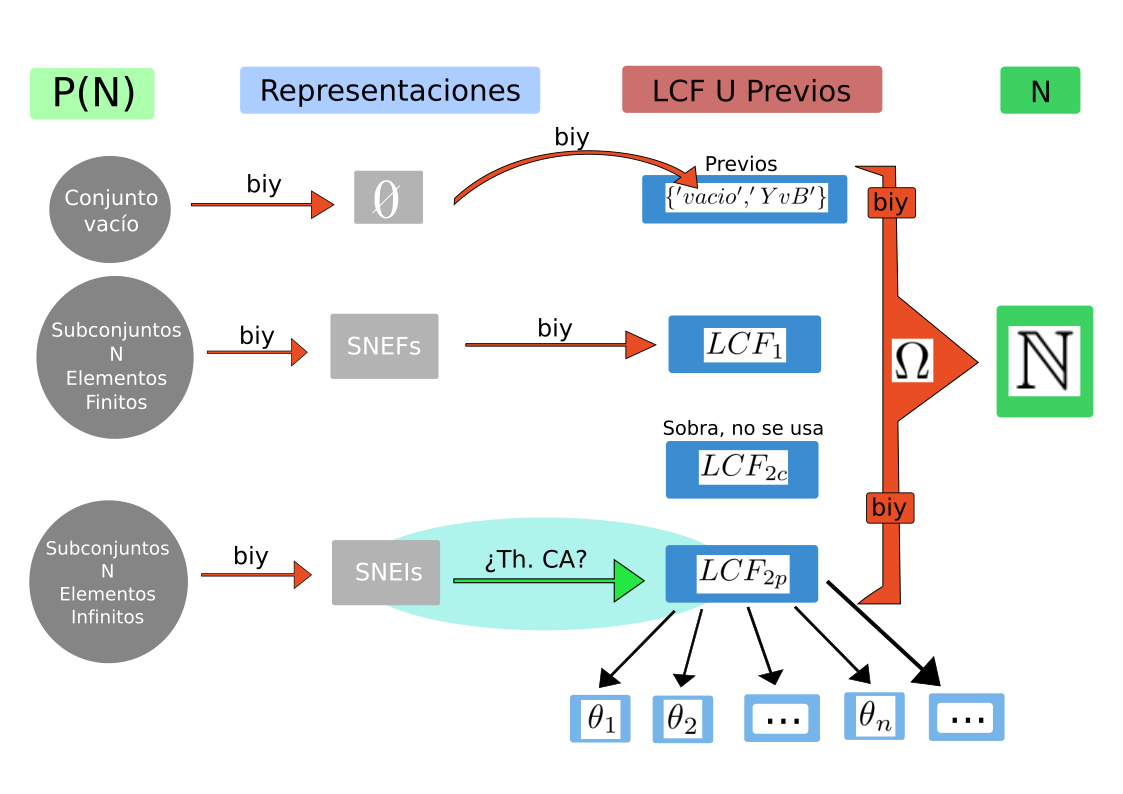
\includegraphics[ scale=0.7, angle=90]{EsquemaRelaciones}
		%\includegraphics[width=\textwidth, scale=0.3]{Funcion_hx_002_v4}
		%\includegraphics[width=\textwidth, scale=0.3]{Funcion_hx_001_v4}
		\centering
	\end{figure}

\newpage
\section{Definiciones}
\subsection{Cadenas de subconjuntos y particiones}
\subsection{SNEF}
\subsection{SNEI}
\subsection{LCF U previos}



\newpage
\section{Sentido cardinal de las soluciones multiverso}

\subsection{Variante de la función definida por partes}
\subsection{Fenómeno real}

En realidad, tratar de explicarlo como una variante de la función definida por partes es sólo una forma de tratar de adaptar el concepto real de mi cabeza a algo que le pueda sonar a un matemático.

Es más bien... como si en una situación de pelea, un grupo fuesen solo dos personas, y el otro veinte personas. De tal forma, que el segundo grupo puede asignar 10 personas a cada persona del primer grupo.

Llamemos grupo de pelea PN al formado por dos personas, y grupo de pelea N al formado por 20 veinte personas. N puede crear dos "Packs" de diez individuos cada uno. Un Pack para cada miembro de A. La proporción es 1 a 10.

De repente, la gente del grupo N, decide quitar 3 miembros de cada Pack. Así que ahora la proporción desciende a, 1 a 7. Por cada miembro de PN hay 7 miembros de N en la pelea.

Luego en otro arrebato de 'indecisión', la gente del grupo N decide quitar dos miembros más de cada Pack. Ahora la proporción de la pelea es de 1 a 5.

UNA VEZ MÁS... en otro arrebato de indecisión... la gente del grupo N, decide quitar un miembro de cada Pack... y la proporción baja a 1 a 4.

El grupo PN sigue en inferioridad numérica!! A pesar de todos los cambios de opinión sobre como crear los Packs, antes de la pelea.

Lo gracioso, quizás por culpa de no saber explicarme bien... es que hay gente que me ha dicho algo equivalente a esto:

PN tiene un cardinal mayor que N, porque no paras de cambiar de opinión, eso es un indicativo de que estás equivocado y que PN, "tiene" (ojo, "tiene", y no "no tiene") un cardinal mayor que N.

Cuando todavía N sigue teniendo una proporción 1 a 4... y la gente del grupo PN está superada en número de forma clara.

El truco "para dudar infinitas veces" es crear Packs de tamaño infinito... y asegurarte de que siempre que quitan un grupo de elementos... esta sustracción consista, siempre, en una cantidad finita de elementos. Contando las sustracciones anteriores acumuladas. Si por muchas veces que quites 'algo', las sustracciones acumuladas, son de un total de elementos de cardinal finito, sea cual sea, siempre nos van a sobrar infinitos elementos en cada Pack. Dejando N a PN, en una clara situación de desventaja. PN siempre estaría superado en número, de forma... infinita... en proporción infinita: 1 a infinito. A través de todas las infinitas 'indecisiones'.   

Nuestro problema consistirá en que tenemos infinitos Packs.. no uno solo, por cada miembro. Cada Pack "intentará" ser disjunto con todos los demás Packs. La misma persona de N... no 'peleará' con dos personas distintas del otro grupo PN. Cada Pack con infinitos miembros. Por cada miembro de PN, no vamos a tener infinitos miembros de N. Vamos a tener infinitos Packs, y cada Pack va a tener infinitos miembros de N.

Para comprobar esto bastaría con chequear todos los posibles pares de miembros de PN. Si en algún posible par, solo uno, de entre todos los Packs asignados a cada miembro del par, encontramos un solo miembro en común, repetido, habríamos fracasado en nuestro intento.

Y lo que va suceder va a ser terriblemente curioso. Partimos de afirmar que podemos crear Packs disjuntos para cada miembro de PN. Pero como ya dije, en vez de un solo Pack por cada miembro, crearemos varios Packs: infinitos Packs, realmente.

Y va a suceder que van a encontrar pares de miembros de PN, cuyos Packs, tienen miembros en común. PERO, simplemente quitando una cantidad finita de Packs, de nuestra asociación, los Packs restantes, volverán a ser disjuntos, para ese par.

Se podrá volver a encontrar otros pares... formados incluso por algún miembro del par anterior... que tengan, ahora, con la nueva asignación, después de haber quitado algunos Packs... miembros en común. PERO no pasará nada: quitando otra vez una cantidad finita de Packs, de todos los posibles pares, no solo arreglaremos estos nuevos pares, sino también los anteriores que hayamos mencionado, volviendo a tener todos, una cantidad infinita de Packs, disjuntos entre sí... 'por ahora'.

Hasta que alguien encuentre un nuevo par... quitaremos una cantidad finita de Packs, y los primeros pares, los anteriores y los actuales... volverán a dejar de tener miembros de N en común. 

DE esta forma, el 'por ahora' es eterno y completo. No existirá NINGÚN PAR, que nos impida seguir teniendo, infinitos Packs, con infinitos elementos cada uno, 'aparentemente disjuntos entre sí', si solo observamos los pares actuales, y todos los que quiera que se nos hayan ocurrido en el pasado, sin tener en cuenta su cardinal. Sin tener en cuenta la cantidad de pares que hayas preguntado en el pasado.

Para todo, PARA TODO, posible par, SIEMPRE, nos quedarán 'más allá' Packs, de los infinitos iniciales, de sobra, que NO crean conflictos con miembros en común.

En realidad no estamos reasignando elementos. Al igual que el ejemplo inicial, no reasignamos, quitamos unos, y DEJAMOS OTROS sin tocar que estaban ahí desde el inicio. Manteniendo todo el rato la proporción de desventaja de PN sobre N.

Y al conjunto PN, le resultará imposible encontrar un par, o una lista de pares, que nos obliguen a quitar TODOS los packs.

Excepto en un único caso... solo cuando haya usado TODOS los posibles pares, SOLO usando TODOS, sin dejarse ni uno, podrá dejarnos vacío el conjunto de Packs disponibles.

No es que use unos, y le sobren algunos pares... debe usar el poder combinatorio de absolutamente TODOS sus pares. De tal forma, que a la vez que nos deja vacío el conjunto de Packs disponibles... su conjunto de pares capaces de 'crear conflictos' también debe vaciarse. La única opción que tiene, es generar una situación de doble derrota. De doble vaciamiento de posibilidades... al renunciar a TODAS sus posibilidades, ojo , a TODAS, para poder vaciar nuestro conjunto de Packs disponibles.

Creándose un extraño empate, que genera situaciones muy curiosas.

Primero. La frustrante situación de verse superado uno a infinito constantemente.

Segundo. La única forma de evitarlo es aceptar un empate: Ni PN tiene pares capaces de dejar vacío el cojnunto de Packs de cada miembro de PN, ni N tiene un conjunto de Packs capaz de cubrir todos los posibles pares, por sí solo.

Tercero. Para cada posible par, SIEMPRE hay infinitos Packs disponibles que resuelven su conflicto. Y no como casos aislados... para ese par, y todos los anteriores que se te pudiesen haber ocurrido. En realidad incluso más, pero eso lo explicaremos con más detalle más adelante.

Cuarto. Que aunque sea un empate, es un empate de poder de combinatoria, bajo el handicap de siempre mantener la proporción 1 a infinito, no 1 a 1. Y recordemos que el poder de combiantoria e sun indicativo del cardinal de un conjunto.

Quinto. Que podemos replicar a la inversa estos fenómenos en las diagonalizaciones de Cantor. Podemos vaciar el conjunto de 'elementos externos construíbles', a pesar de que para biyección, exista un elemento externo, al igual que para cada posible par, existe, siempre, digamos... un universo capaz de generar Packs disjuntos para ese par. Y ENCIMA, podemos construir una diagonalización inversa. Si PN tiene un cardinal mayor que N, debe existir un par de miembros de PN que tengan en sus Packs, elementos en común. Pero ese par no existe... negando la primera frase. Siempre tengo disponibles una serie de Packs, más allá de los que quitamos para hacer los pares disjuntos. Así que el razonamiento es incorrecto o tenemos una contradicción.




